\documentclass[12pt]{article}
\pagestyle{empty}
\usepackage{amsmath,times,bm,hyperref}
\usepackage{amssymb}
\usepackage{stmaryrd}
\usepackage{graphicx}
\usepackage{listings}
\usepackage{xcolor}
\lstset { %
    language=C++,
    backgroundcolor=\color{black!5}, % set backgroundcolor
    basicstyle=\footnotesize,% basic font setting
}

%%%%%%%%%%%%%%%%%%%%%%%%%%%%%%%%%%%%%%%%%%%%%%%%%%
% Do not modify the dimensions of the page
\setlength{\topmargin}{0mm}
\setlength{\headheight}{0mm}
\setlength{\headsep}{0mm}
%% 25.4 -25.4 = 0
\setlength{\topmargin}{0mm}
%% 25.4 -25.4 = 0
\setlength{\oddsidemargin}{0mm}
%% 210 -25(left) -25(right) = 160
\setlength{\textwidth}{160mm}
%% 297 -25(top) -30(bottom) = 242
\setlength{\textheight}{242mm}
\setlength{\parindent}{0pt}
\setlength{\parskip}{12pt}
% Do not modify the dimensions of the page
%%%%%%%%%%%%%%%%%%%%%%%%%%%%%%%%%%%%%%%%%%%%%%%%%%

\begin{document}

\begin{center}
% TITLE: replace text with your abstract title WITHOUT full stop
\textbf{\Large
Homework 3
}\\
\normalsize Due April 13 2021

% AUTHOR/AFFILIATION: handled by authblk. 
% Use only one of the two following methods for author listing. Delete or comment out the other.
% Add/remove authors/affiliations as necessary, complete following the template without adding additional superscript/footnotes  

% 1- Authors have the same affiliation:
% ~~~~~~~~~~~~~~~~~~~~~~~~~~~~~~~~~~~~


%%%%% AFFILIATIONS %%%%%

\end{center}
\begin{enumerate}
\item Let $\bm S$ be a second-rank tensor and $\bm T$ be a symmetric second-rank tensor. Prove that
\begin{align*}
S_{ij} T_{ij} = S_{(ij)}T_{ij} = S_{(ij)}T_{(ij)}.
\end{align*}

\item (Euler-Lagrange condition of the Galerkin formulation) 
\begin{enumerate}
\item Consider the weak-form problem of the one-dimensional model problem,
\begin{align*}
\int_0^1 w_{,x} u_{,x} dx = \int_0^1 w f dx + w(0)h,
\end{align*}
in which $w$ and $u$ are assumed to have sufficient smoothness \textit{globally}. One can show its equivalence to the strong-form problem via considering its Euler-Lagrange condition. Now we consider the corresponding Galerkin formulation, where the test function and trial solution are represented by piecewise linear functions. Therefore, they are smooth only in the element interiors, but are only $C^0$ across element boundaries. Because of this, we can only perform integration-by-parts in an element-by-element fashion for the Galerkin formulation. Show that
\begin{align*}
0 =& \sum_{A=1}^{n}\int_{x_A}^{x_{A+1}} w^h \left( u^h_{,xx} + f \right)dx + w^h(0)\left( u^h_{,x}(0^+) + h \right) \\
&+ \sum_{A=2}^{n} w^h(x_A)\left( u^h_{,x}(x^{+}_A) - u^h_{,x}(x^{-}_A)\right).
\end{align*}
Further, show that the above Euler-Lagrange condition suggests that
\begin{align*}
& u^h_{,xx} + f = 0, \quad \mbox{ for } x \in (x_A, x_{A+1}), \mbox{ and } A = 1, 2, \cdots, n, \\
& -u^h_{,x}(0^{+}) = h, \\
& u^h_{,x}(x^{-}_A) = u^h_{,x}(x^{+}_A), \quad \mbox{ for } A = 2,3,\cdots, n.
\end{align*}

\item Consider the weak-form problem for elastostatics,
\begin{align*}
\int_{\Omega} w_{(i,j)} \sigma_{ij}d\Omega = \int_{\Omega} w_i f_i d\Omega + \int_{\Gamma_h} w_i h_i d\Gamma.
\end{align*}
If the test and trail function spaces are constructed by $C^0$ basis functions, show that
\begin{align*}
0 = \sum_{e=1}^{n_{el}} \int_{\Omega^e} w^h_i \left( \sigma^h_{ij,j} + f_i \right)d\Omega - \int_{\Gamma_h} w^h_i \left( \sigma^h_{ij}n_j - h_i \right) d\Gamma - \int_{\Gamma_{\mathrm{int}}} w^h_i \llbracket \sigma_{ij}n_j\rrbracket d\Gamma,
\end{align*}
wherein
\begin{align*}
\Gamma_{\mathrm{int}} := \cup_{e=1}^{n_{el}} \partial \Omega^e - \partial \Omega.
\end{align*}
From the above Euler-Lagrange equation, one may readily conclude that the Galerkin formulation implies
\begin{align*}
& \sigma_{ij,j} + f_i = 0, && \mbox{ in } \cup_{e=1}^{n_{el}} \Omega^e, \displaybreak[2]\\
& \sigma_{ij}n_j = h_i, && \mbox{ on } \Gamma_h, \displaybreak[2]\\
& \llbracket \sigma_{ij}n_j\rrbracket = 0, && \mbox{ on } \Gamma_{\mathrm{int}}.
\end{align*}
\end{enumerate}

\item(Voigt notation) 
\begin{enumerate}
\item Show that $\bm \sigma^{\mathrm{vect}} = \bm D \bm \epsilon^{\mathrm{vect}}(\bm u)$ is equivalent to $\sigma_{ij} = c_{ijkl} \sigma_{kl}$.
\item Show that $w_{(i,j)} c_{ijkl} u_{(k,l)} = \left( \bm \epsilon^{\mathrm{vect} }(\bm w)\right)^T \bm D \bm \epsilon^{\mathrm{vect}}(\bm u)$.
\item For isotropic materials, setup the matrix $\bm D$.
\end{enumerate}


\item Use quadratic and linear shape functions to design shape functions for the six-node quadrilateral depicted in the following figure. Write a pseudo-code (or draw a flow chart) that calculate the basis functions and their derivative values at a given quadrature point.

\begin{figure}[h]
	\begin{center}
	\begin{tabular}{c}
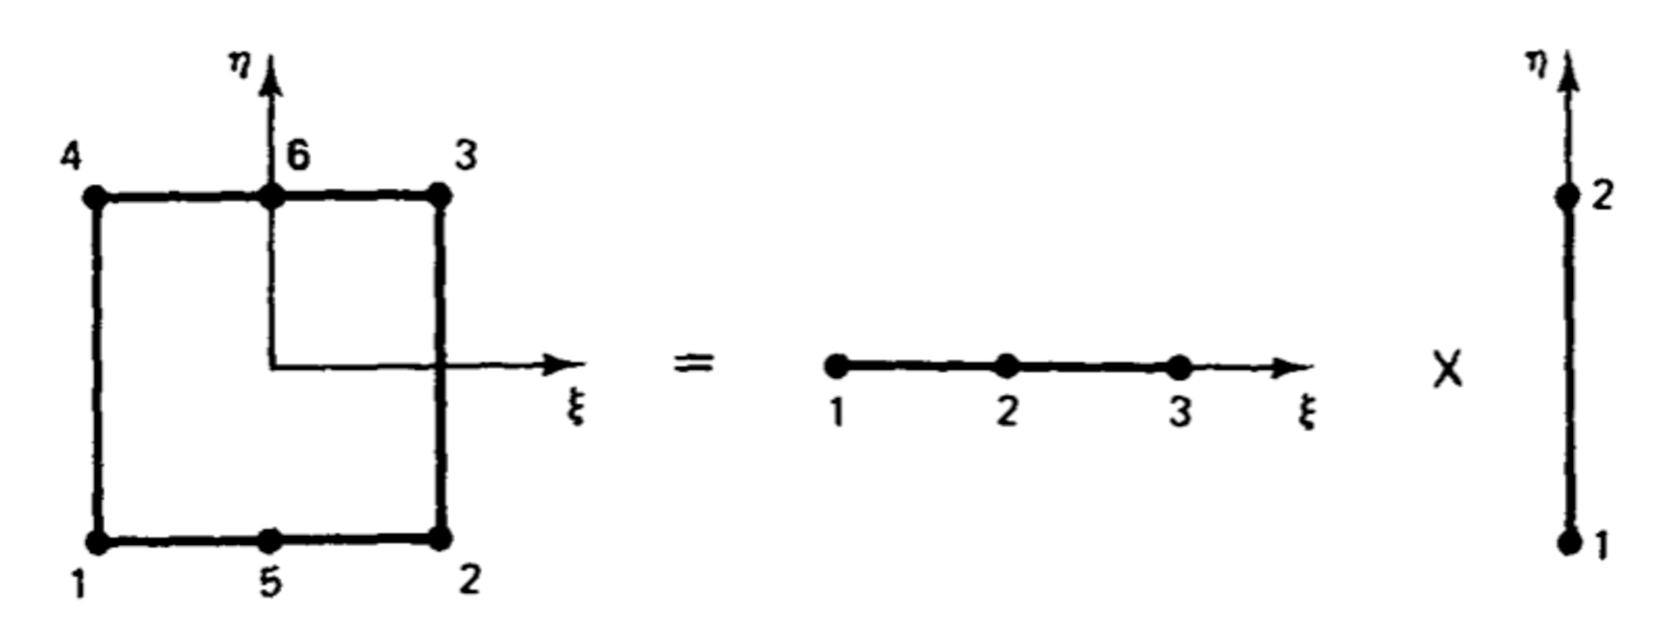
\includegraphics[angle=0, trim=0 0 0 0, clip=true, scale = 0.35]{./6node-elem.pdf}
\end{tabular}
\end{center} 
\label{fig:quad_elem}
\end{figure}

\item(Final projects stage 1: Design your problem) Select one of the analysis problems listed below as your final project topic. Here are some possible problems for the project.
\begin{itemize}
\item Bernoulli-Euler beam and Timoshenko beam theories;
\item Solve plane-strain incompressible materials using the mixed finite element method;
\item Three-dimensional thermal analysis;
\item Plane-strain elastodynamic analysis;
\item Plane-strain linear visco-elasticity analysis;
\item Solve Helmholtz equation via the p-version finite element method;
\item Your own project (discuss with me).
\end{itemize}
You are encouraged to work with teammates. Each team is allowed to have 1, 2, or at most 3 members. At this stage, you need to decide your project topic and setup your team. In this homework, you shall report (1) your project topic and (2) your team members.

A few more words about the final projects: Final projects will be reported by a in-class presentation (10 minutes) and a written report. A report shall include the following contents.
\begin{itemize}
\item Problem description: Describe the objective of the analysis. Describe the physical model to be analyzed and the overall engineering assumptions, material properties, loading conditions, etc.
\item Design of the numerical methods: Describe the weak-form problem, the finite element technology chosen, the Galerkin formulation, and the matrix problem.
\item FEA code: A brief summary of the finite element program and a complete set of numerical codes that can reproduce your results.
\item Results and analysis: Include methods that you use to verify the correctness of your code. Include important results and a discussion should be accompanied these results.
\item Conclusions: Describe what has been learned from the analysis and what conclusion can be drawn.
\end{itemize}
The importance of a thorough documentation and judicious use of appendices cannot be overemphasized. Reports should include enough detail that an experienced analyst could completely reproduce the results from reading the reports alone.
\end{enumerate}

\end{document}

